\chapter{System Design and Implementation}

This chapter describes of the system. It starts by providing overview of the system, followed by requirement elicitation to build prototype. Furthermore, it also provide deeper understanding of architectural paradigm by discussing each module and their interconnection.

\section{Overview}

Pervious chapter limits our discussion about the design decision and describe the essential component of the system.  Since the concept is quite abstract and does not dictate any implementation details.  In order to challenge the relevance and capability of the concept, a prototype app, tailored to a real world scenario, should be developed as a “proof of concept”. Our system is divided in to two components: (1) Rest based web application follows modular principle of system design i.e. functionality of a system is divided into multiple concurrent modules. Where coordination of modules depend on database.  Each module has its own Data Access Object (DAO) through with communication take place. Module query existing data with the help of DAO perform their task and update afterward. (2) iOS client provides all the required interface to communicate with the server. It aims to collect information that needs to build user profile and allow active learning and critiquing mechanism to update user profile and increase the trust between user and system by conveying the idea how much system cares about user and his need. 

\section{Requirment elicitation}

This section represents user’s viewpoint of the system. It also describes the purpose of the system by identifying the Functional, non-functional requirements and description of use case in the form of scenarios. It is important to mention here that all the scenarios are developed to evaluate the prototype and are not meant for production purpose. 

\subsection{Functional Requirments}

FoodForMe is a mobile food recommender system that user iOS platform. It purpose to facilitate user to find the food what to cook that matches their personal preferences. Idea behind this prototype application is to proof the concept a combination of Persuasion and critique-based recommender system lead to better recommender and have an impact on user decision making process. Therefore all the functionality in a design is bounded to this purpose. There are two cases of interaction with the system. In case one user need login via Facebook so that system can get its demographic profile instead of asking him to fill out his personal information. Demographic information contains name, birthday, email, name and link of his profile picture. By default system keeps his cooking time preference and course selection preference. User can change these preferences from the setting screen. In second case user can interact without login and having same default preference. As it is notice that some user hesitate to provide their information without having a trust in a system. However, in this particular case user can only view the information. Our rest of discussion will relate do case one.\newline

After getting login and change his preference. User will able to view recipes according to his preference. Each recipe shows the name, star rating, main categories, sub categories, number of reviews and recipe picture. Once the user tap on any recipe, user is able to view detail of selected recipe. Detail screen consists on 3 to 4 sections depends on screen type. Section 1 contains the generic information about the recipe same as discuss above accept it provide large Image of recipe. In Section 2 is related to recipe ingredients, each ingredient item have its name and quantity. Section 3 is about preparation/direction means its guide user how to cook that recipe. Section 4 is an option selection and it will appear as per screen type. In this section system will provide why system think this recipe is according to user preference. User is able to see two screens that display recipes list. First one will display the popular recipes of the system. Recipe course and popularity are the factors on which this will depends on. Motivation behind this to aware user what’s new and hot in system and allow user to change his taste. On the other hand second list will depends only user preference. On detail screen of each recipe system will provide explanation, which tells user what system will think about him and why these recipe recommend to him. \newline

On the detail screen of selected recipe user can criticized on showed item. User can critique on list of indigents by mentioning them he like that ingredient or not. Also he might be able to critique on recipe by given star according to his choice. Additional system allow user to change his personal preferences these include cooking time and course selection. \newline


\subsection{Non Requirments}

From usability to performance aspect of a system Non-functional requirement can apply in many ways. However it is our assumption that this app is a prototype and will only use for evaluation purpose but we have to consider User interface, performance and supportable requirements \cite{burigat2005bringing}. Following are some few non-functional requirements that should guide to development process:

\begin{enumerate}

	\item App must not be crash.
	\item Any mobile user can use the application and have a clear understanding of app without facing any problem.
	\item App should provide consistence user interface with respect to colors, fonts and theme.
	\item App should follow the Application User interface guideline provided by apple.
	\item For app start to critiquing or selection of preference must be reachable at any time.
	\item Processing time of app may not exceed to 1 second. 
	\item Server calls should not take more 30 sec.

\end{enumerate}

\subsection{Use-Cases}

Figure \ref{fig:ch4_use_case_foodforme} illustrates foodforme uses cases.  These include login via Facebook, user can change his preference according to his convenience, browsing of recipes, critiquing on recipe based on ingredients and rating and selection of recipe to cook. To discuss the use cases we follow the scenario approach \cite{bruegge2004object}.

\begin{figure}[h]
	\centering
	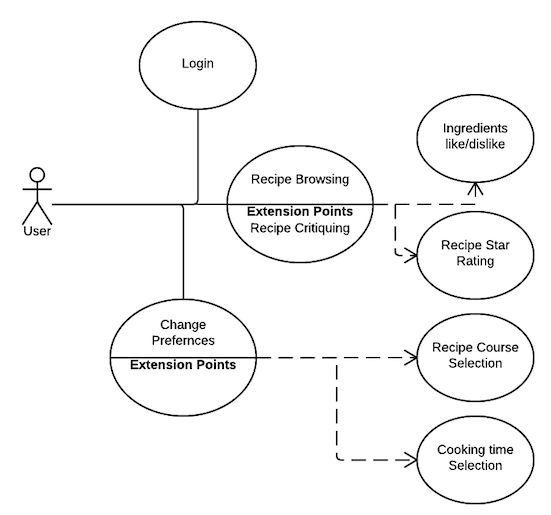
\includegraphics[width=.5\linewidth]{figures/ch4_use_case_foodforme.png}
	\caption{FoodForMe use case diagram}
	\label{fig:ch4_use_case_foodforme}
\end{figure}


\section{System Architecture}

\subsection{Working}

\subsection{Class Drigram}

\subsection{ERD}

\section{System Services}

\subsection{Service 1}
